\documentclass[12pt]{article}
\usepackage{listings}
%\usepackage[utf8]{inputenc}
\usepackage{inputenc}
\usepackage{graphicx}
\usepackage{float}
\usepackage{array}
\lstset{
extendedchars=\true,
language=JAVA,
%inputencoding=utf8,
%basicstyle=\ttfamily,
%basicstyle=\ttfamily\fontsize{8}{8},
%commentstyle=\ttfamily\fontsize{8}{8},
basicstyle=\tiny;
columns=fullflexible,
%xleftmargin=5pt,
frame=single,
breaklines=true,
postbreak=\mbox{{$\hookrightarrow$}\space},
}
\renewcommand{\thesubsubsection}{\alph{subsubsection} )}
%\renewcommand{\thesubsubsection}{\thesubsection.\alph{subsubsection} )}

\begin{document}

\title{Addon zu den Übungsaufgaben I, SBV1 }
\author{Lisa Panholzer, Lukas Fiel}
\maketitle


\newpage
\section{Übungsaufgaben I, addon}
\subsection{Stressanalyse}

\subsubsection{Recherche}

\subsubsection{Analyse der EKG Sequenzen}

\subsubsection{Herzratenvariablität}

\subparagraph{Analyse des Hautleitwerts}

\subsection{Geschwindigkeitsermittlung}
\label{sec:Geschwindigkeitsermittlung}
\subsubsection{Ermittlung von Geschwindigkeit und Distanz}
\textit Aufgabenstellung:
Zu untersuchen war ein Datensatz, der mit Daten eines Beschleunigungssensors gefüllt war. Neben den Daten des Sensors waren auch Zeitstempel enthalten mit denen eine Ermittlung der Abtastzeit möglich war. Bekannt war weiters, dass es sich um die Daten einer geradlinigen Bewegung entlang einer Tischkante handelte die etwa 2 m lang war. Eine Darstellung dieser Daten kann Figure \ref{fig:plainData} entnommen werden.

\begin{figure}[H]
	\centering
	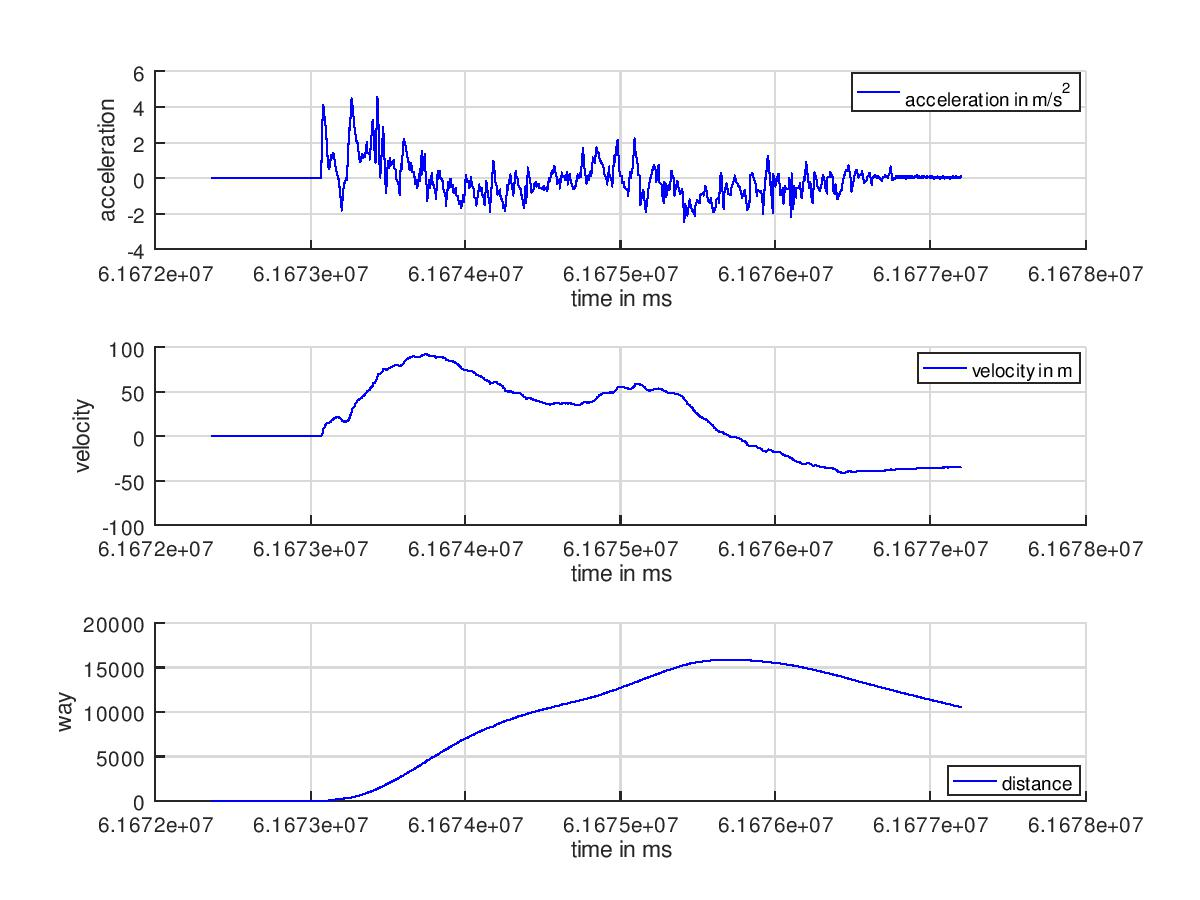
\includegraphics[width=12cm]{images/testData.jpg}
	\caption{Die Daten des Beschleunigungssensors wurden aufsummiert um die Geschwindigkeit zu erhalten. Dieser Prozess wurde wiederholt um einen ersten Eindruck über ein mögliches Wegsignal aussehen könnte.}
	\label{fig:plainData}
\end{figure}

\begin{figure}[H]
	\centering
	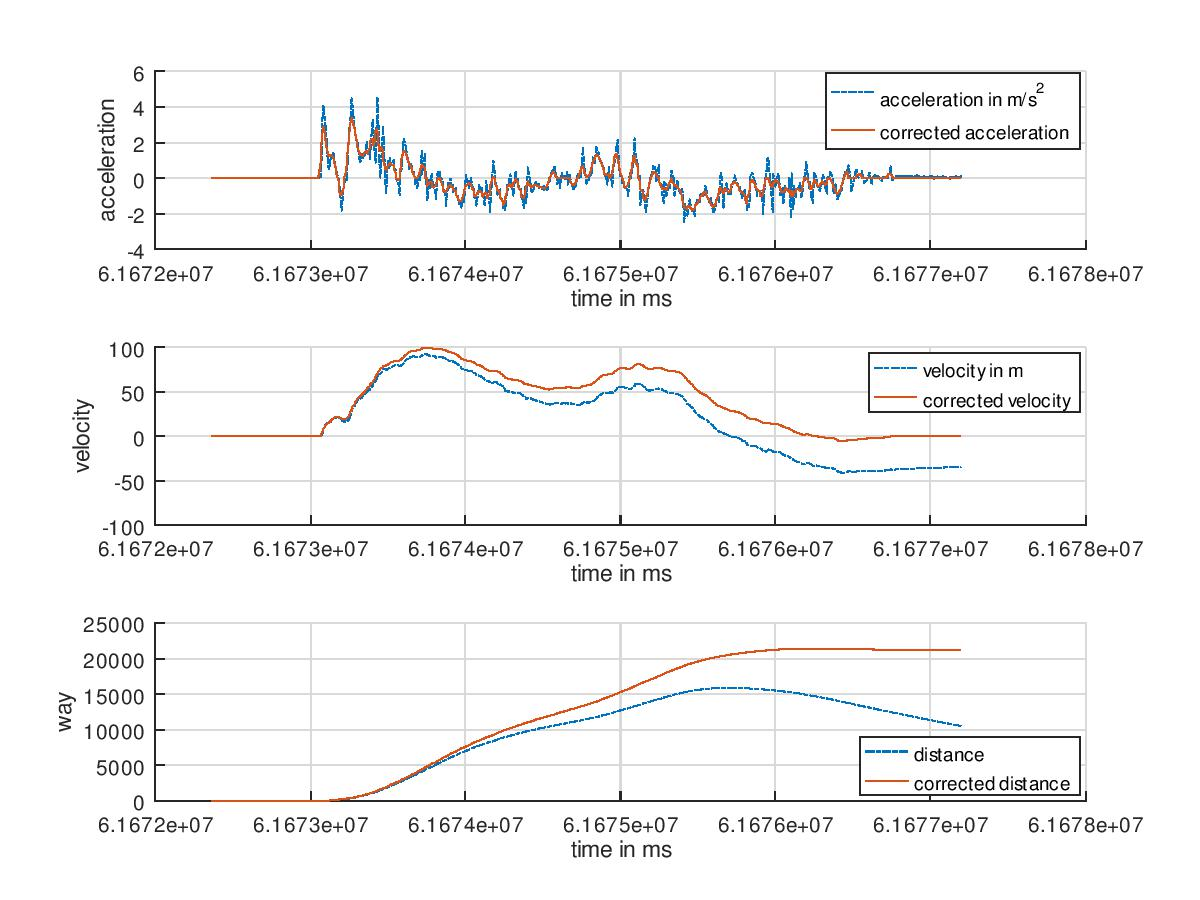
\includegraphics[width=12cm]{images/filteredData.jpg}
	\caption{Gefilterte und korrigierte Darstellung der Daten.}
	\label{fig:filteredData}
\end{figure}


\lstinputlisting[frame=single,breaklines=true]{../accelerometerProcessing.m}

\end{document}
